\chapter{Исследовательская часть}

\section{Интерфейс приложения}

На рисункe  \ref{fig:interface} приведено изображение интерфейса приложения.

\begin{figure}[h!]
	\centering{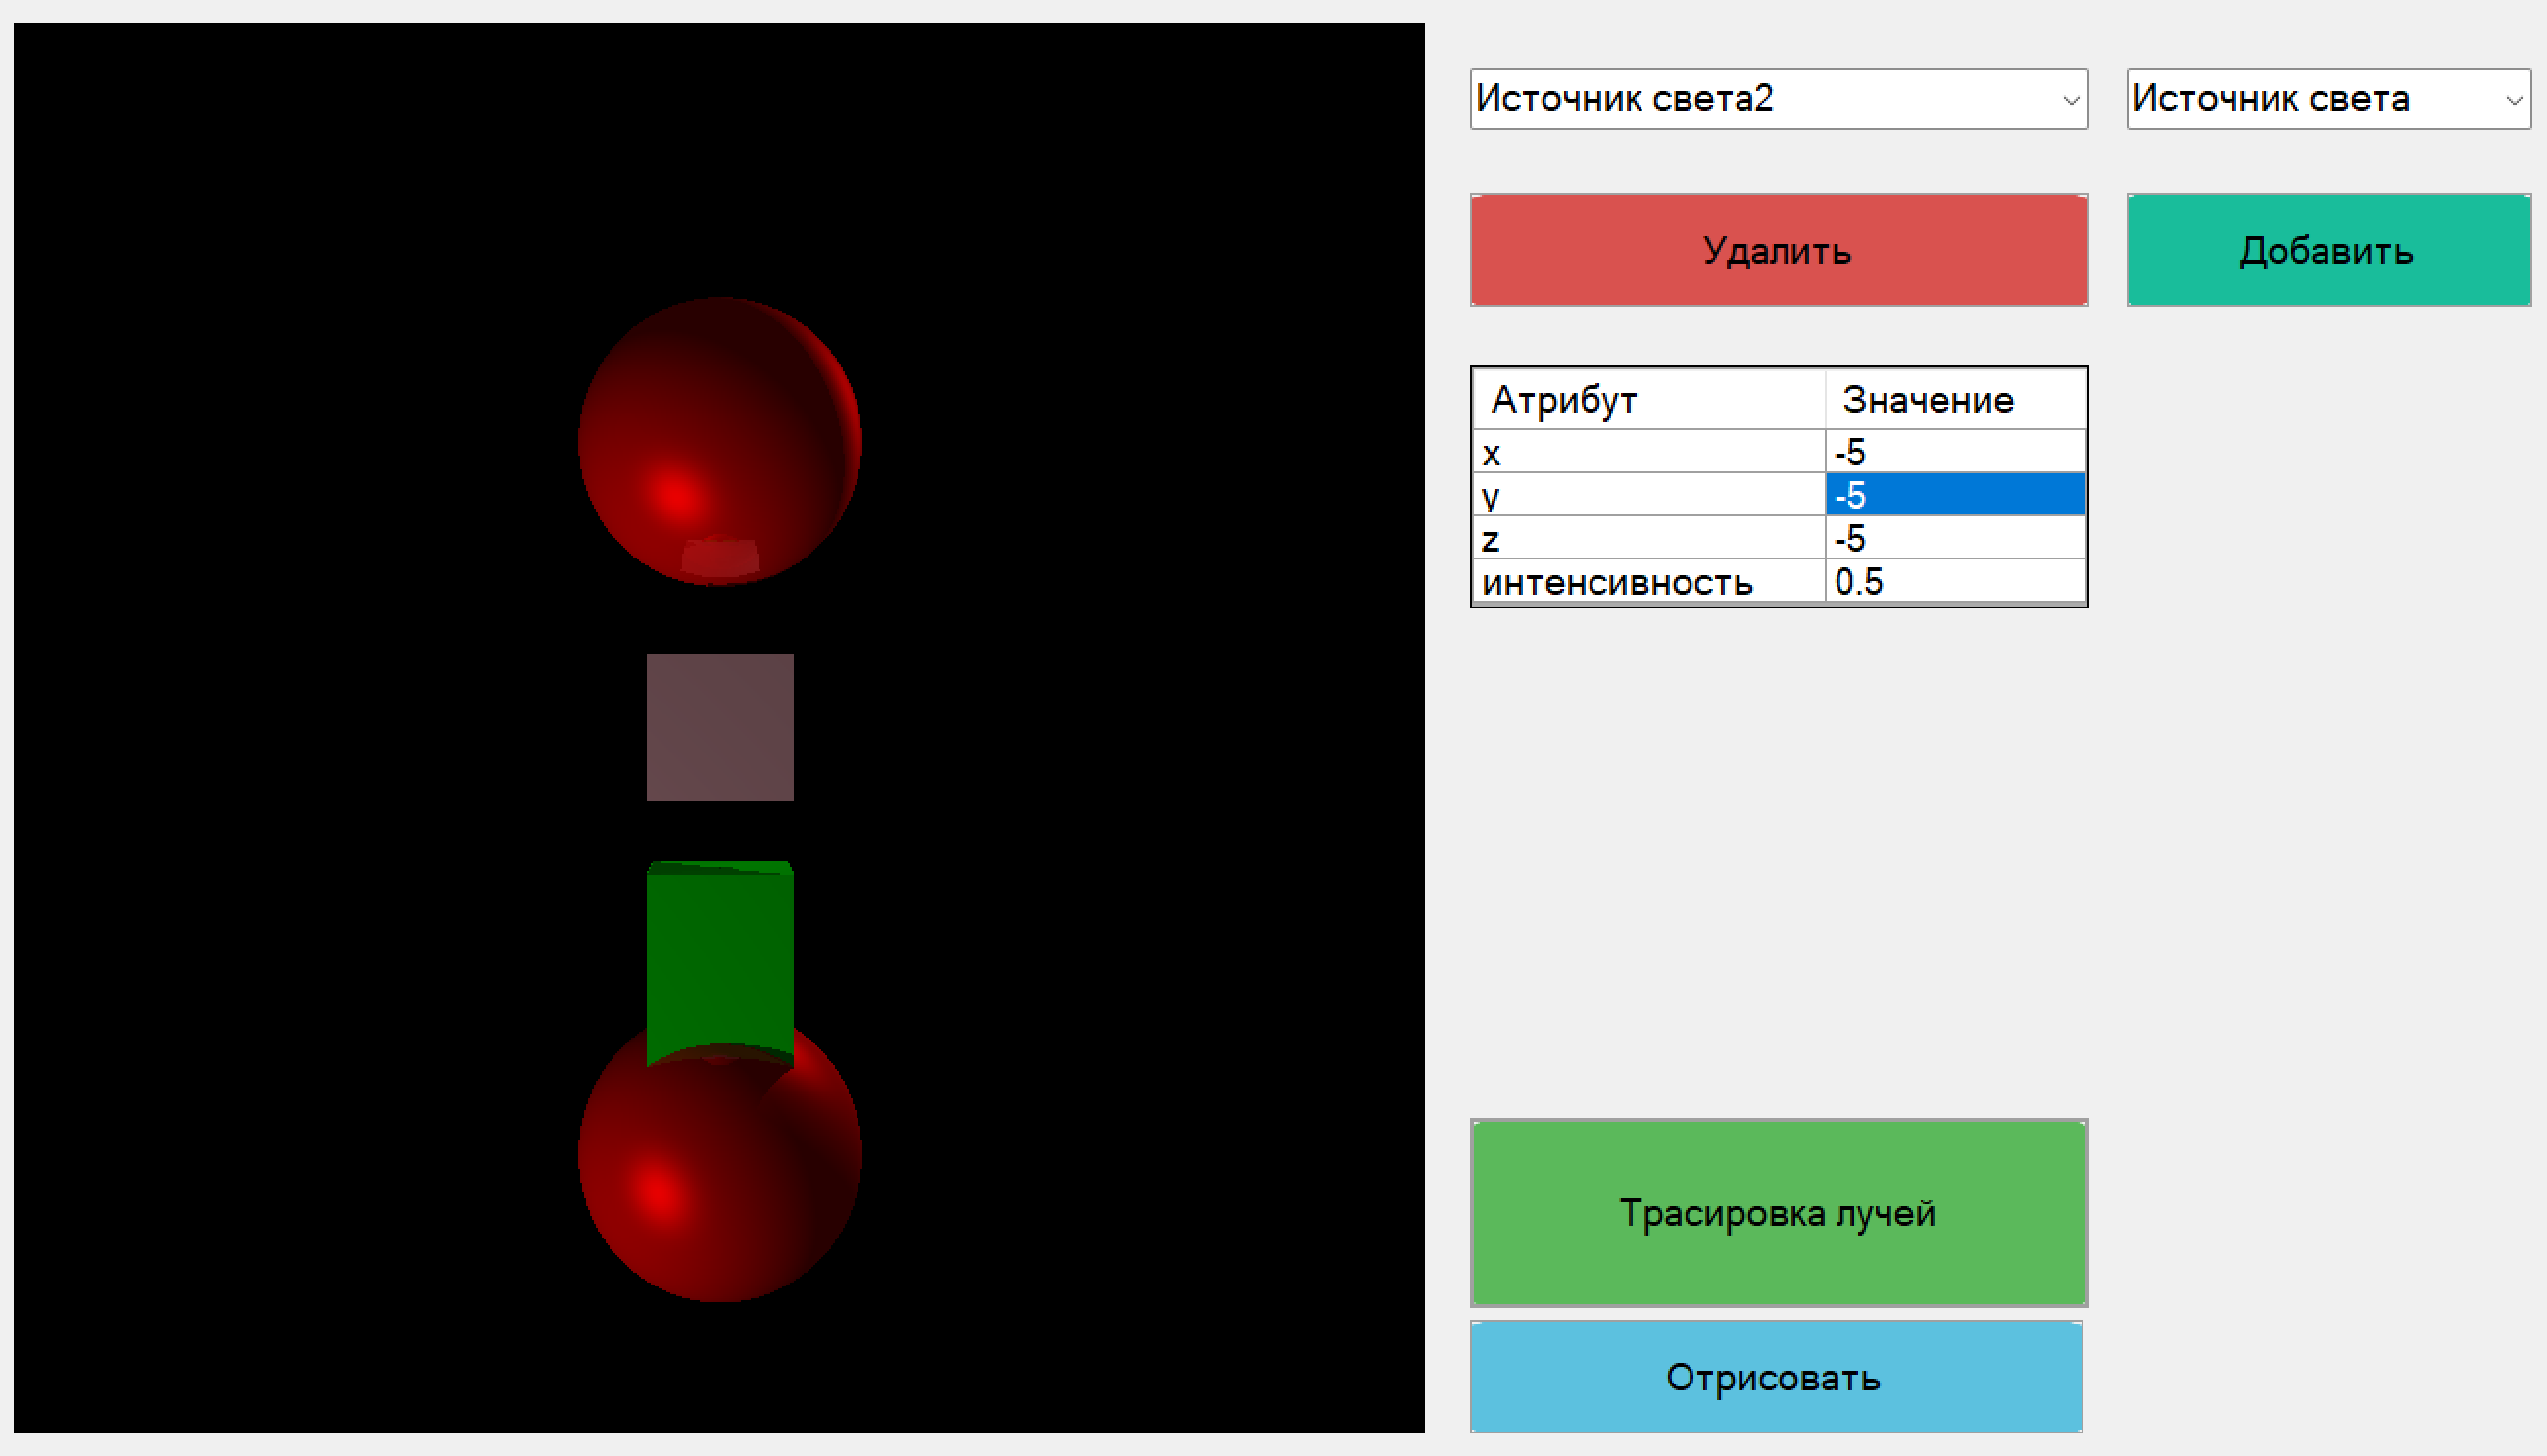
\includegraphics[scale=0.5]{photos/interface.png}}
	\caption{Интерфейс}
	\label{fig:interface}
\end{figure}

\section{Сравнение реализаций трассирования лучей}

В процессе выполнения курсового проекта были реализованы два метода трассировки лучей. 
Реализация этих методов различается по сложности. 
Для удобства их идентификации им были присвоены названия: простой и модифицированный. 
Простой метод отличается от модифицированного тем, что не учитывает тени, зеркальность объектов и их гладкость.
Необходимо провести сравнение времени выполнения каждого метода в зависимости от количества объектов на сцене.

Для проведения сравнения между указанными алгоритмами были созданы специальные сцены, включающие в себя различное количество объектов.

На рисунке~\ref{fig:graph} приведен график, на котором отображается зависимость времени выполнения алгоритмов от количества объектов на сцене.  Время построения сцены рассчитывалось как среднее значение из 20 измерений.
\begin{figure}[ht!]
	\begin{center}
		\captionsetup{singlelinecheck = false, justification=centerfirst}
		\begin{tikzpicture}
			\begin{axis}[
				xlabel={Количество объектов},
				ylabel={Время в секундах},
				width = 0.95\textwidth,
				height=0.43\textheight,
				xmin=0, xmax=50,
				ymode=log, 
				legend pos=north west,
				legend style={font=\footnotesize},
				xmajorgrids=true,
				grid style=dashed,
				]
				
				\addplot[
				blue,
				semithick,
				mark = *,
				mark size = 3pt,
				thick,
				] file {graph/normal_raytrace.csv};
				
				\addplot[
				red,
				semithick,
				mark = *,
				dashed,
				] file {graph/modified_raytrace.csv};
				
				\legend{
					Простой алгоритм обратной трасировки лучей,
					Модифицированный алгоритм обратной трасировки лучей
				}
			\end{axis}
			
		\end{tikzpicture}
		\centering
		\caption{Сравнение времени работы реализаций алгоритмов}
		\label{fig:graph}
	\end{center}
\end{figure}

\section*{Вывод}
Явно заметно, что простая реализация требует меньше времени в сравнении со модифицированной. 
Однако следует учитывать, что простой алгоритм не полностью справляется с задачей создания реалистичного изображения. 
Простой алгоритм отлично подходит для работы со сценой, добавления объектов, изменения их свойств и прочего. 
Как только все объекты установлены и изменены, можно запустить модифицированный алгоритм для получения более реалистичного изображения.